\documentclass[12pt]{extarticle}
\usepackage[utf8]{inputenc}
\usepackage{amsmath}
\usepackage{hyperref}
\usepackage{float}
\usepackage{graphicx}
\usepackage{caption}
\usepackage[export]{adjustbox}
\usepackage{amssymb}
\usepackage{hyperref}
\usepackage{algorithm}
\usepackage{algpseudocode}
\usepackage{multirow}
\usepackage{listings}
\usepackage{xcolor}
\lstset { %
    language=C++,
    backgroundcolor=\color{black!5}, % set backgroundcolor
    basicstyle=\footnotesize,% basic font setting
}

\newcommand{\quotes}[1]{``#1''}

\title{SPM project - JACOBI}
\author{Luca Moroni (635966)}
\date{- 2022}

\linespread{1.2}
\usepackage[a4paper,margin=1in,footskip=0.25in]{geometry}


\begin{document}

\maketitle

\section{Analysis}
In this section will be considered the theoretical analysis on the paralallelization of the \textbf{Jacobi} algorithm.\\
As first step I design the pseudocode of the Jacobi Iterative Method, Algorithm \ref{alg:jim}.
\begin{algorithm}
\caption{Jacobi Iterative Method}\label{alg:jim}
\begin{algorithmic}[1]
\Require $A \in \mathbb{R}^{n \times n}$ (strictly dianogally dominant), $b \in \mathbb{R}^n$, max\_iters (max number of iterations), $\epsilon$ (optimality tollerance).
\Ensure $x \; s.t. \; Ax = b$

\State $x^{prev} \gets \{0\}^n$
\State $x^{k} \gets \{0\}^n$

\State $k \gets 0$

\While {True}
    \For {$i \gets 1$ to $n$}
        \State $\sigma \gets 0$
        \For {$j \gets 1$ to $n$}
            \If {$j \neq i$}
                \State $\sigma \gets \sigma + A_{i, j} * x^{prev}_j$
            \EndIf
        \EndFor
        \State $x^k_i \gets \frac{(b_i - \sigma)}{A_{i,i}}$
    \EndFor
    
    \State $k \gets k+1$
    \If {$k = max\_iters$}
        \State break
    \EndIf
    
    \If {$\| x^k - x^{prev} \|_2 \leq \epsilon$}
        \State break
    \EndIf
    
    \State $x^{prev} \gets x^{k}$
\EndWhile
\end{algorithmic}
\end{algorithm}
We can notice that the external loop (lines 4-22) have to be done sequentially, due to the fact that the $x^{k+1}$'s elements depend to the elements of $x^k$. On the other hand the two internal loops can be computed in a parallel fashion, the first \texttt{for} (line 5-13) can be totally parallelized, due to the independence in the computations done for $x_i^k$ and $x_j^k$ for $i$ and $j$ different at same iteration $k$. Due to the property of independence just stated we can parallelize the first \texttt{for} statement using a map pattern apply as function the computations done in the body, this kind of data-parallel pattern is coherent with our problem since the data is availavable at the start of the first \texttt{for}.\\
Analyzing again the code we can notice, moreover, that the internal for (lines 7-11) can be parallelized, the computations can be done with a reduce parallel pattern, the reduce variable is $\sigma$, the operation is the sum, that is commutative and associative (mandatory requirements for an operation to be used in a reduce pattern) and the elements of the data-parallel pattern consist in $a_{ij}x_j^k$.\\
Even the computation of the norm of the vectors difference (line 18) could be parallelized, using the map pattern to do the element-wise square difference and the reduce pattern to do the summation of map's resulting vector.\\
In practice, I choose to not implement the reduce pattern in the case of the internal \texttt{for}, due to the fact that the overhead would be too large and the grain too small, even the norm computation will be computed in a sequential fashion since it wont affect the order of magnitude of the sequential fraction and it will be negligible when $N$ is large.\\
Since other published works (e.g. \cite{margaris2014parallel}) do experiments without taking into account the distance stopping criteria (lines 18-20), I have implemented two kinds of runs, the one that compute the norm computation and use the distance as stopping criteria and the other that don't do it.\\\\
First of all I implemented the sequential version of the code, same as reported in this presentation, this kind of implementation is mandatory to have the time necessary to run the sequential code, necessary for the computation of the metrics used in the experimental phase.\\
For the experiments done I used the \textbf{speedup}, the \textbf{scalability} and the \textbf{efficiency} metrics.\\\\
We can analyze and decompose the Time of the sequential version of Jacobi Iterative Method,
\[T_{seq\_jacobi}(N) = T_{init\_vars}(N) + M(N*T_{jacobi\_iteration}(N) + T_{norm}(N)),\]
where $M$ are the iterations needed to converge, $N$ is the dimension of the problem, $T_{jacobi\_iteration}$ is the time needed to execute the function parallelized (lines 6-12) and $T_{init\_vars}(N)$ is the time needed to initialize necessary variables (lines 1-2).\\ 
Latency of the map pattern is defined in the following way,
\[T(map(f, nw)) = \frac{N}{nw}t_f + t_{split} + t_{merge},\]
where the $nw$ is the number workers and $N$ is the dimension of the problem, $t_f$ is the time needed to compute the function of a single element (in our case a single iteration of the first \texttt{for} (lines 6-12), $t_{split}$ is the overhead time to split the data among the those and $t_{merge}$ is the overhead time needed to merge the results from the workers.\\
Assuming that We will be in Shared Memory scenario the time needed to distribute the data to the workers and the time needed to collect the results will not have a huge impact.\\
Assuming moreover that, the threads can be forked and joined outside the while loop (line 4), the parallel Jacobi's time can be modelled as,
\begin{equation*}
\begin{aligned}
T_{par\_jacobi}(N, nw) = T_{init\_vars}(N) \; + T_{fork}(nw) + T_{join}(nw) \; + \\ M[\frac{N}{nw}*T_{jacobi\_iteration}(N) \; + \; T_{split}(nw) + T_{merge}(nw) + T_{norm}(N)]
\end{aligned}
\end{equation*}
For the implementations that doesn't use the distance the times' computations are the same but without $T_{norm}(N)$ in the formulae above.\\\\
Before to pass to the implementation section we can compute the serial fraction of our problem ($f = \frac{serial \; operations}{total \; operations}$), taking into account only the order of magnitude of the operations:
\[f \approx \frac{(M*N) + K}{M*(N^2 + N) + K} \; ,\]
where $M$ is the steps necessary to converge and $N$ is the problem dimension, and $K$ represent the order of magnitude of the memory and workers allocations or preliminary operations, such as swapping vectors, $K$ in practice is at most of the order of $N$ (assuming that $N \geq nw$), the operations (apart the second \texttt{for}) in the \texttt{while} loop are at most of the order of $N$ (e.g. norm computation), so,
\[f \approx \frac{(M*N) + N}{M*(N^2 + N) + N} = \frac{M*(N + \frac{N}{M})}{M*((N^2 + N) + \frac{N}{M})} = \frac{N*(1 + \frac{1}{M})}{N*(N + 1 + \frac{1}{M})} = \frac{1 + \frac{1}{M}}{N + 1 + \frac{1}{M}}\]
This is a very crude approximation. In the implementation in wich the norm is not computed the factor $N$ in the numerator will have a lower impact, so the parallelization might have more effect since the effective serial fraction will be lower. We will see those aspects in the experimental phase.\\
With the serial fraction we can exploit the Amdahl law (strong scaling) and the Gustafsson law (weak scaling) to analyze the results of our experiments.\\
For the Amdahl law we have that $\textbf{speedup}(n_w) \leq \frac{1}{f} \approx \frac{N+1}{2}$, for a given $N$.\\
For the Gustafson law we have that $\textbf{speedup}(n_w) = n_w - (n_w - 1)*f \approx n_w - (n_w - 1)*(\frac{2}{N + 1})$.\\
Those computations are useful to see that the serial fraction is inversely proportional to the dimension of the problem and from the Amdahl (or Gustaffson) rule we can say that the speedup will have a better values (as a function of number of workers) for larger $N$.
\section{Implementation}
I implemented four version of the Jacobi Iterative Method:
\begin{itemize}
    \item \textbf{Sequential}: Simple c++ implementation of the pseudo-code showed in the previous section.
    \item \textbf{Fast Flow}: Apply the same logic of the Native Threads implementation but using the Fast Flow's api.
    \item \textbf{Native Threads (Thread Pool)}: Implementation of the Jacobi algorithm using pthread library following the patterns discussed in the previous section.
    \item \textbf{Native Threads (Barriers)}: Implementation of the Jacobi algorithm using pthread library following the patterns discussed in the previous section.
\end{itemize}

\subsection{Data creation}
We are in a shared memory scenario so the matrix $A$ and the vector $b$ are created and stored in RAM for all the execution. As first step I noticed that the Jacobi method resolution work well and is guarantee to converge when the matrix $A$ is strictly diagonally, so the \texttt{initialize\_problem} function in \texttt{utilis.cpp} take into account this fact, moreover the matrix $A$ and the vector $b$ are created randomly with their components uniformly distribuited in a range $[maximum, minimum]$.
I choose to use the \texttt{vector} class to initialize and store the data due to the simplifications for dealing with, but during the element-wise operation of the Jacobi Iterative Method I casted those vector objets to arrays (contiguous portion of memory, faster to deal with) using \texttt{.data()} method.

\subsection{Sequential Implementation}
For the implementation of the Sequential code there is not to much to be said, the implementation is in the fact the pseudo-code, and can be seen in \texttt{seq\_jacobi.cpp} under the function \texttt{seq\_jacobi\_method}.

\subsection{Fast Flow Implementation}
For the Fast Flow Implementation I used the \texttt{Parallel\_For} class exposed by the library to implement the Map Pattern, the lambda function used in the \texttt{.parallel\_for()} call is implement the \texttt{jacobi\_iteraiton} stated before.\\
\begin{lstlisting}
auto jacobi_iteration = [&](const long i){
    double sigma = 0;

    for (int j=0; j<n; j++) {
        if  ( j!=i )
            sigma = sigma + A_data[i][j]*x_prev_data[j];
    }

    x_k_data[i] = (b_data[i] - sigma)/A_data[i][i];
}
\end{lstlisting}
The instatiation of the \texttt{Parallel\_for} class, is outside the while loop so, in this case as said in the analysis section the overhead of the creation of the threads is done once.\\
The implementation can be seen in \texttt{ff\_jacobi.cpp} under the function     \texttt{ff\_jacobi\_method}.

\subsection{Native Threads Implementation (Thread Pool)}
In the Native thread implementation of the parallelism I used only the pthread classes of C++ standard library. In practice I tryed to write a class with the same semantic of \texttt{Parallel\_for} of Fast Flow, this to implement the Map pattern.\\
The implementation of the parallel for is under the \texttt{th\_jacobi.cpp} in the class \texttt{THParallelFor}, that class is implemented using a Thread pool (implemented in the same file), so when I instatiate the \texttt{THParallelFor} (outside the while loop) I create all the threads waiting the operations to compute. The \texttt{ThreadPool} is a class under the file \texttt{th\_jacobi.cpp} and implement in a generic version a thread pool, this class is based on a SharedQueue used to schedule the messages between the caller and the threads in the pool.\\
The sinchronization time used to deal with a ThreadPool and the SharedQueue is an overhead that can affect the perfomances.\\
The lambda function computed by the single worker in the map fashion computation is the same showed in the Fast Flow implementation.
The implementation can be seen in \texttt{th\_jacobi.cpp} under the function \texttt{th\_jacobi\_method}.

\subsection{Naive Threads Implementation (Barrier)}
Since the straightforward implementation that come into my mind at first glance wasn't the one with the thread pool but the one that use the barriers to synchronize the threads, I also added this implementation.\\
As said this implementation is based over the barrier class, so every thread take its part of the computation and through the external while they are synchronized to wait the termination of all the other threads to terminate the external iteration. the barrier was implemented under the \texttt{th2\_jacobi.cpp} in the class \texttt{MyBarrier}, I implemented the class by my self to deal with hands the code behind this synchronization technique despite since the \texttt{g++-11} the Barrier class is implemented as library class.
The implementation of the Jacobi Iterative Method can be seen in \texttt{th2\_jacobi.cpp} under the function \texttt{th2\_jacobi\_method}.

\section{Experiments}
The experiments aims to see the quality of the parallelization techniques used, to see the \textbf{speedup}, the \textbf{scalability} and the \textbf{efficiency} of the parallel implementations.\\
To do the experiments I tested the sequential, the fast flow and the native threads implementations over two kind of problems that differs for the dimensionality, one with N=1024 (normal size) and the other with N=16384 (huge size), this is useful to see how the solutions scale with the dimensionality and if the theoretical results are correct, the matrices are the same for all the computations, and are initialized with $minimum = -10$ and $maximum = -10$. Moreover I tested the methods differentiating the cases in which the distance criterion is used to stop the method and the case in which only the max number of iteration is used. Remember that we have seen that with larger N the parallelization would have more effect.\\
The experiments are done over a machine with 32 processors with 4 degree of hyperthreading (the max number of workers will be 128) each processor is a: Intel(R) Xeon(R) Gold 5120 CPU @ 2.20GHz.\\
I tested for each of the two dimensions the metrics with growing number of workers, $nw \in [1-128]$, testing for each of $nw$ the time needed to execute the Jacobi Iterative Method over the same matrix (so same operations, same iterations to converge), the times reported are averages over 5 runs, to avoid outliers due to some strange scheduling and other avoidable situations. The max number of iterations are fixed to $5$ in all the runs.

% --- TIMES

\begin{figure}[H]
\centering
    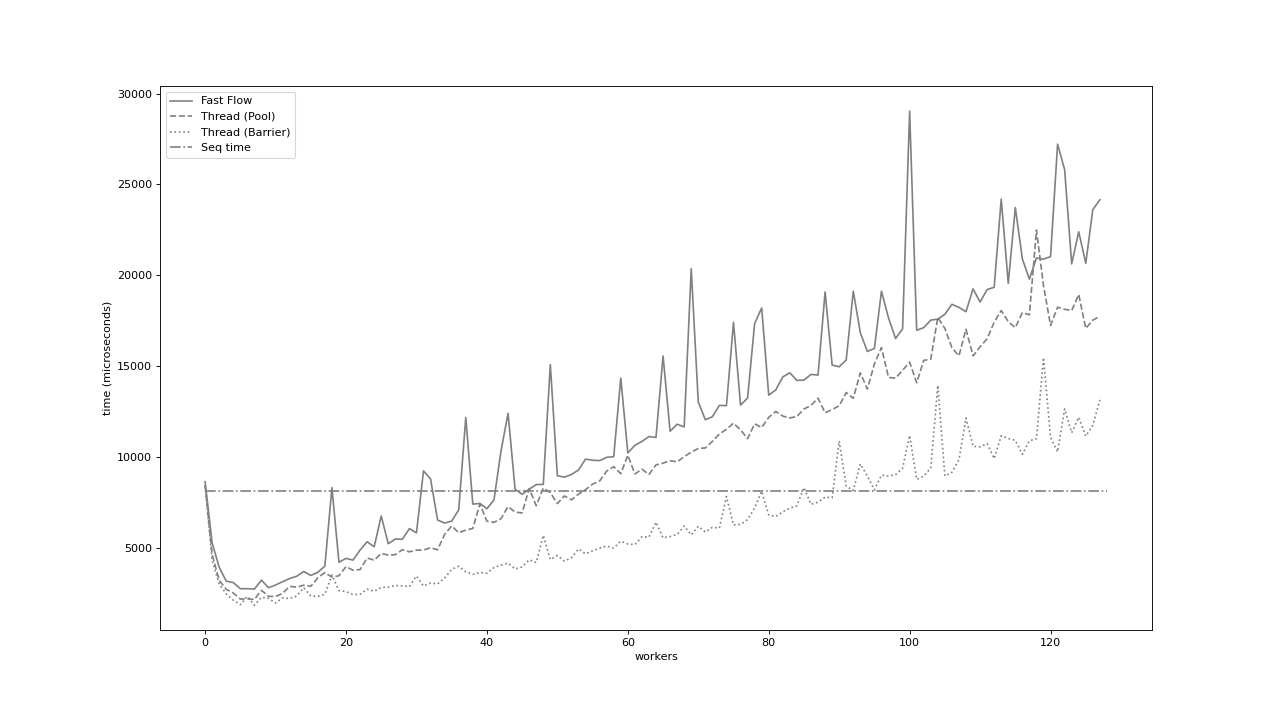
\includegraphics[width=18cm, center]{./plots/times_1024_0.png}
    \caption{Plot of times with n = 1024 without norm computation}
\end{figure}

\begin{figure}[H]
\centering
    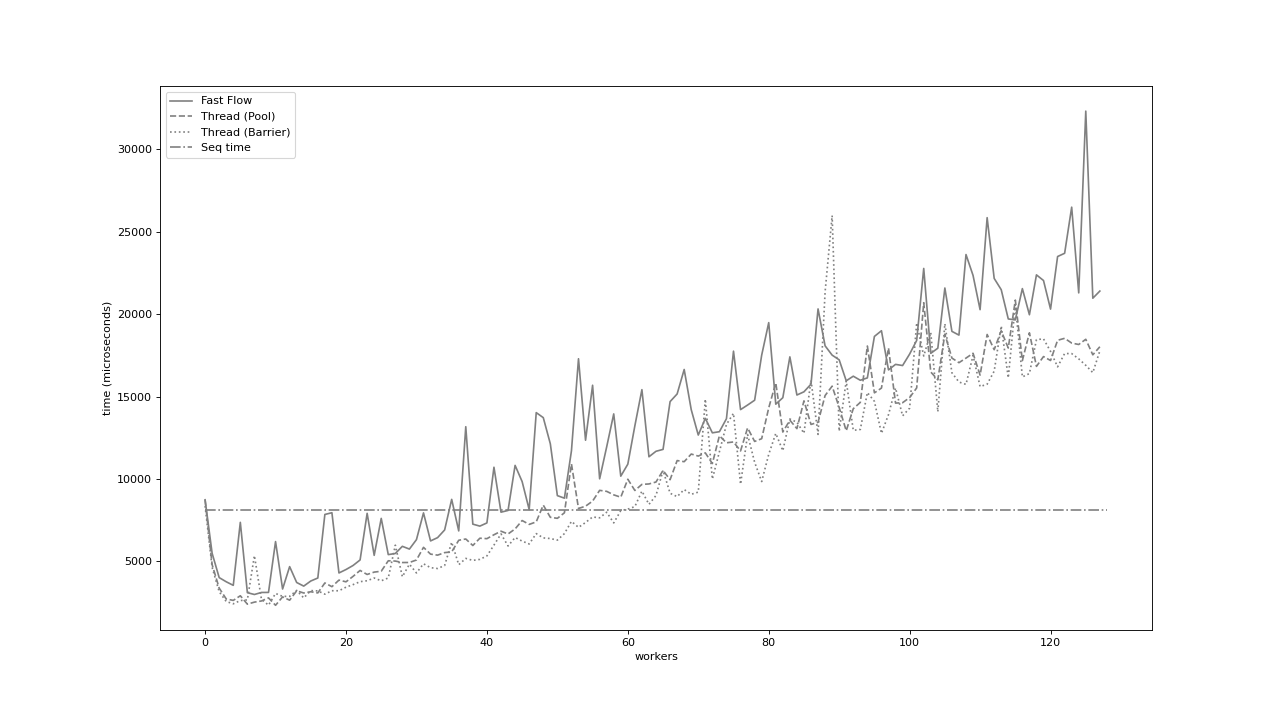
\includegraphics[width=18cm, center]{./plots/times_1024_1.png}
    \caption{Plot of times with n = 1024 with norm computation}
\end{figure} 

\begin{figure}[H]
\centering
    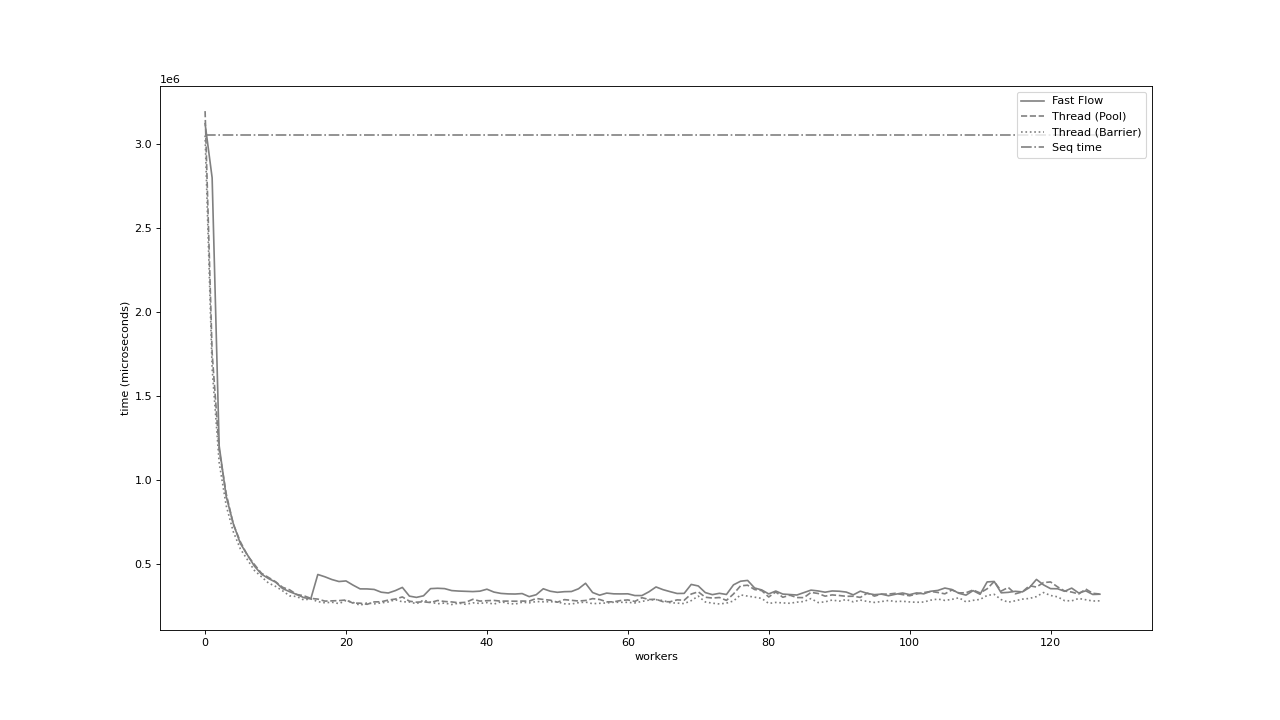
\includegraphics[width=18cm, center]{./plots/times_16384_0.png}
    \caption{Plot of times with n = 16384 without norm computation}
\end{figure}

\begin{figure}[H]
\centering
    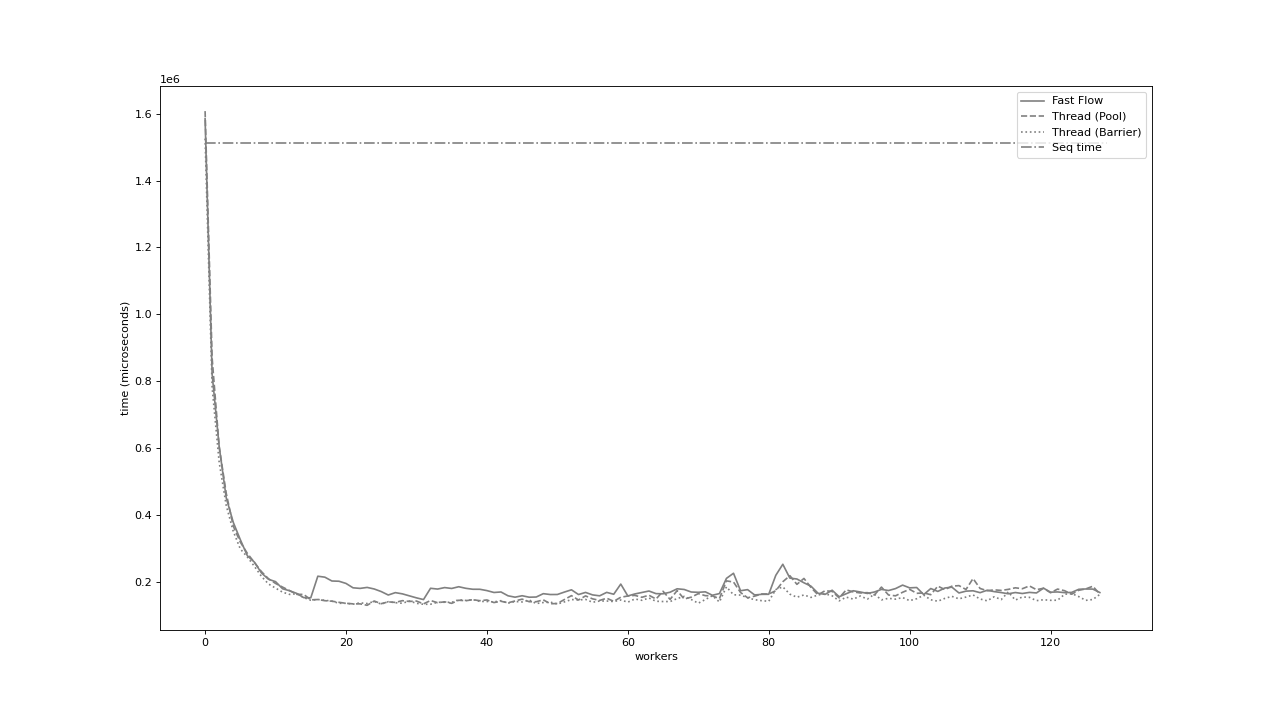
\includegraphics[width=18cm, center]{./plots/times_16384_1.png}
    \caption{Plot of times with n = 16384 with norm computation}
\end{figure}

% --- SPEEDUP

\begin{figure}[H]
\centering
    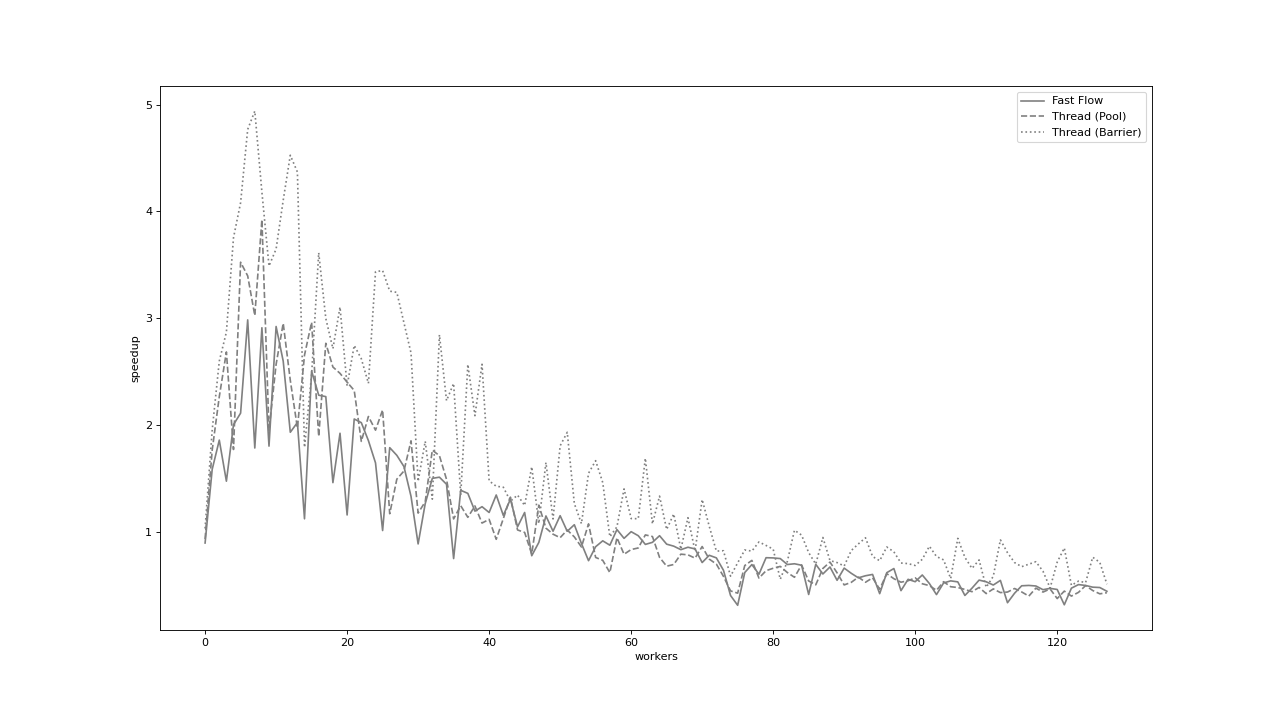
\includegraphics[width=18cm, center]{./plots/speedup_1024_0.png}
    \caption{Plot of speedup with n = 1024 without norm computation}
\end{figure}

\begin{figure}[H]
\centering
    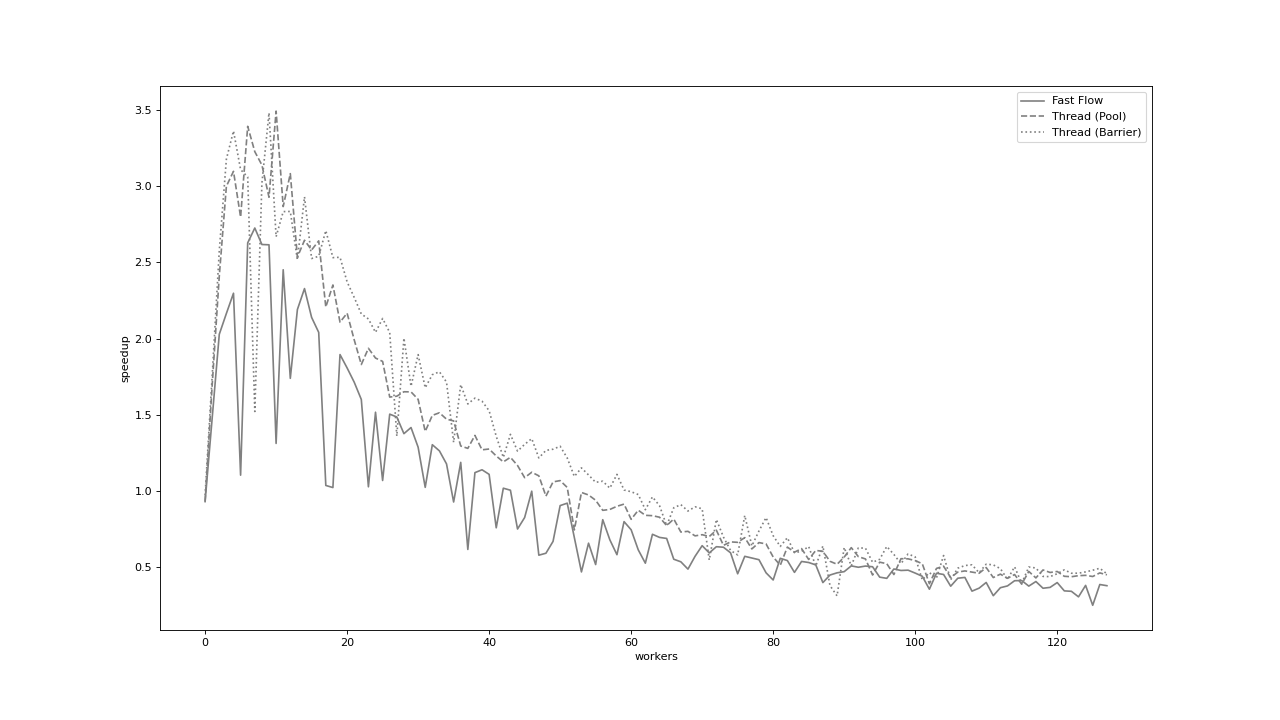
\includegraphics[width=18cm, center]{./plots/speedup_1024_1.png}
    \caption{Plot of speedup with n = 1024 with norm computation}
\end{figure} 

\begin{figure}[H]
\centering
    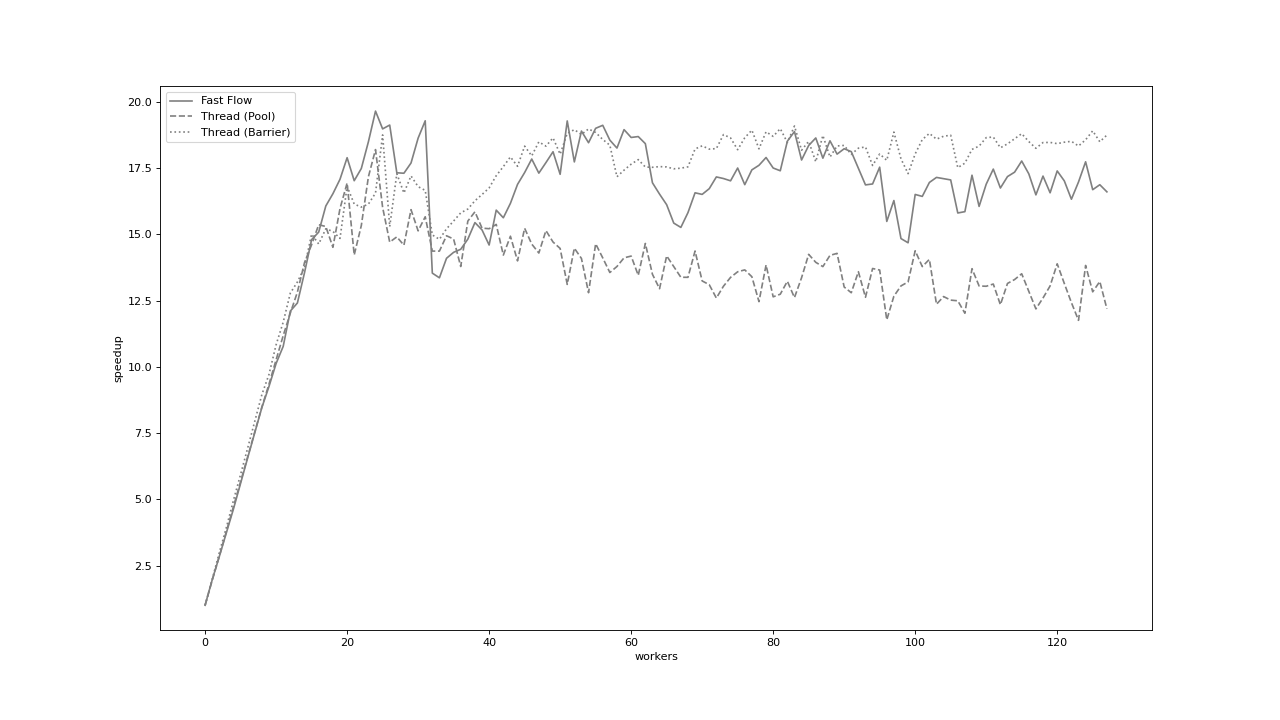
\includegraphics[width=18cm, center]{./plots/speedup_16384_0.png}
    \caption{Plot of speedup with n = 16384 without norm computation}
\end{figure} 


\begin{figure}[H]
\centering
    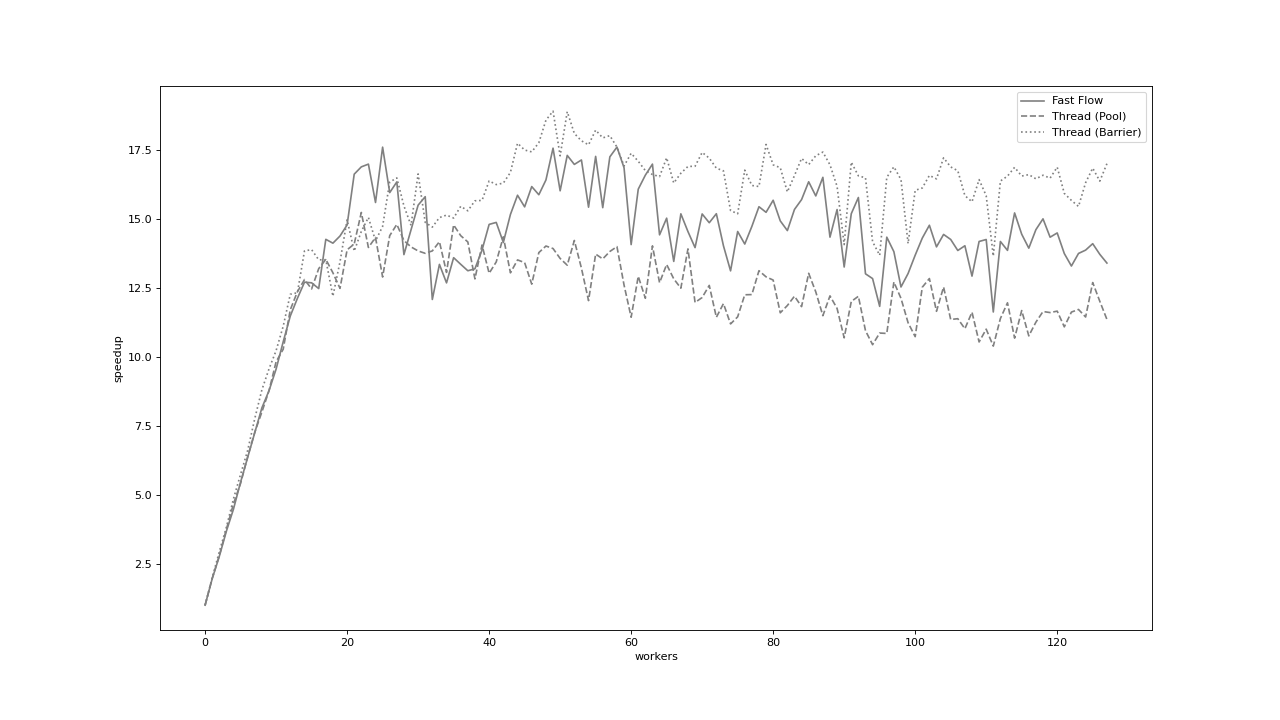
\includegraphics[width=18cm, center]{./plots/speedup_16384_1.png}
    \caption{Plot of speedup with n = 16384 with norm computation}
\end{figure}

% --- SCALABILITY

\begin{figure}[H]
\centering
    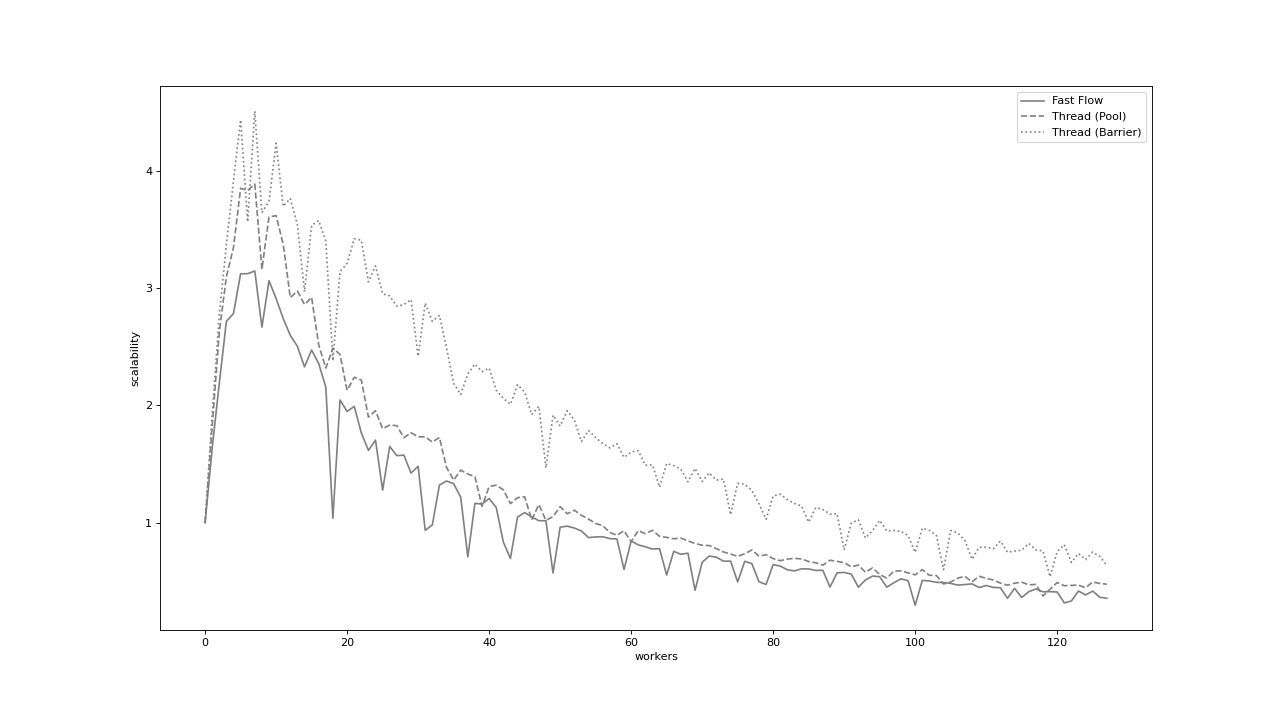
\includegraphics[width=18cm, center]{./plots/scalability_1024_0.png}
    \caption{Plot of scalability with n = 1024 without norm computation}
\end{figure}

\begin{figure}[H]
\centering
    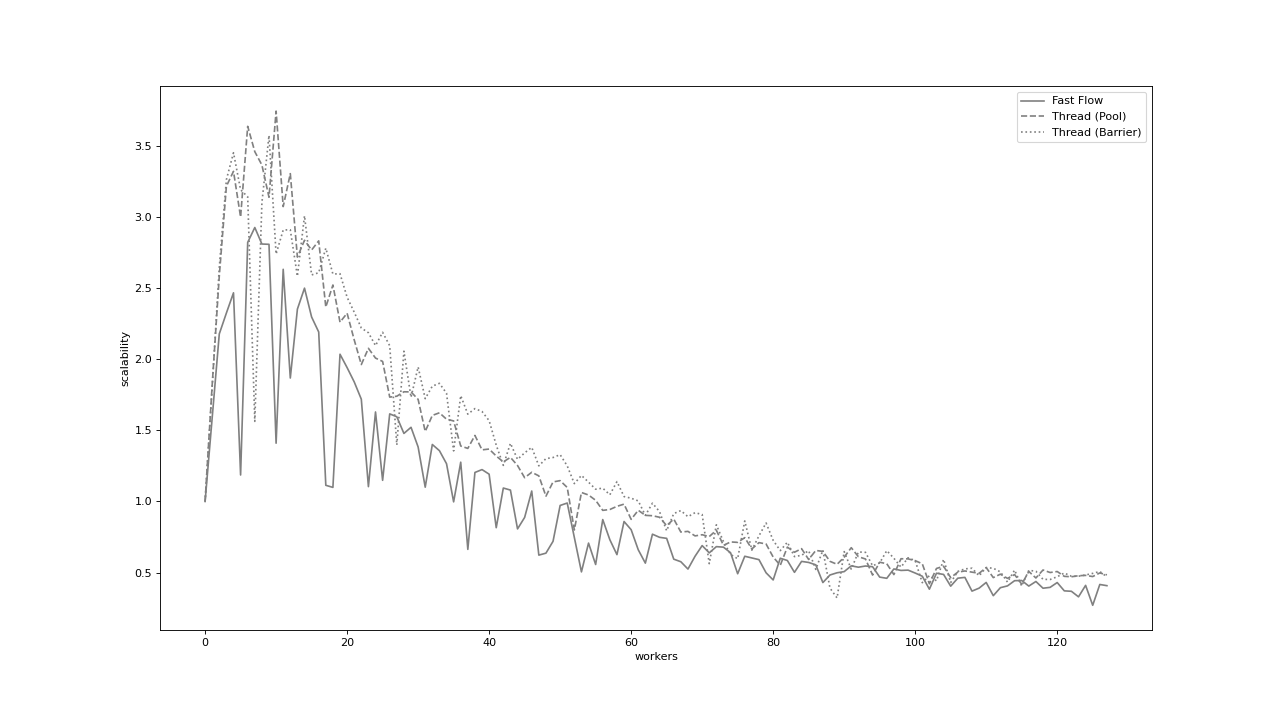
\includegraphics[width=18cm, center]{./plots/scalability_1024_1.png}
    \caption{Plot of scalability with n = 1024 with norm computation}
\end{figure} 

\begin{figure}[H]
\centering
    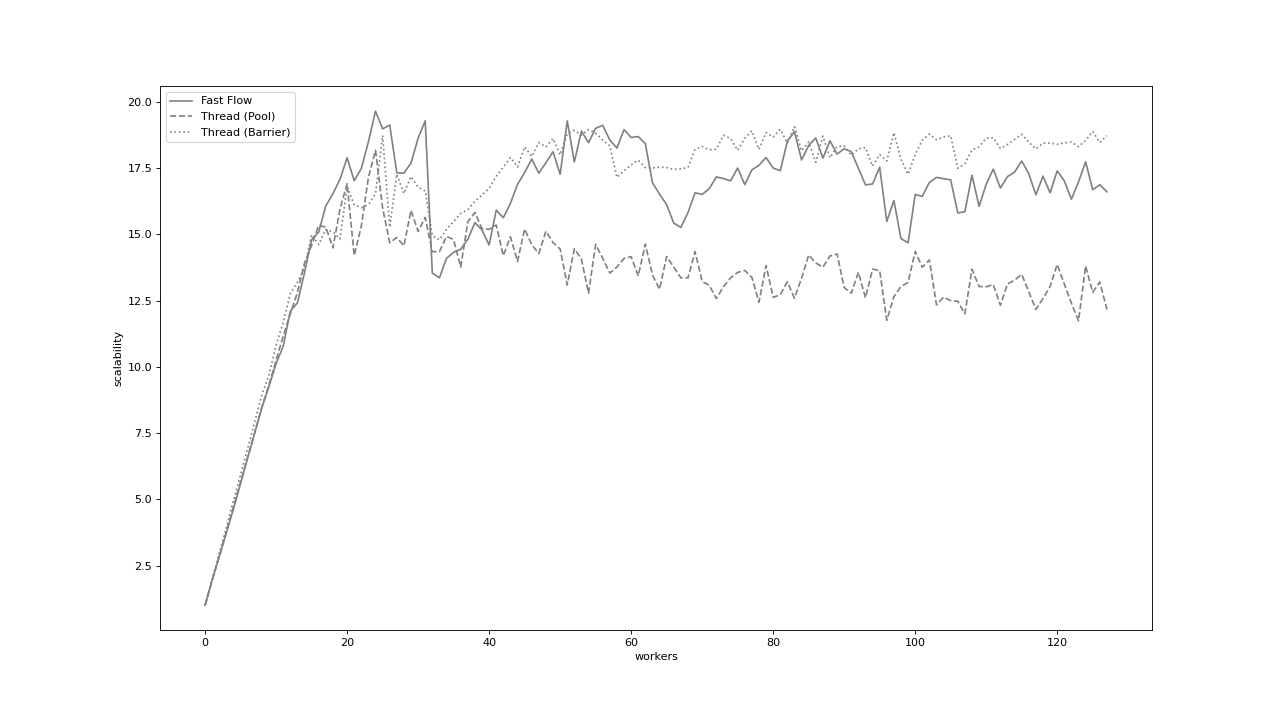
\includegraphics[width=18cm, center]{./plots/scalability_16384_0.png}
    \caption{Plot of scalability with n = 16384 without norm computation}
\end{figure} 


\begin{figure}[H]
\centering
    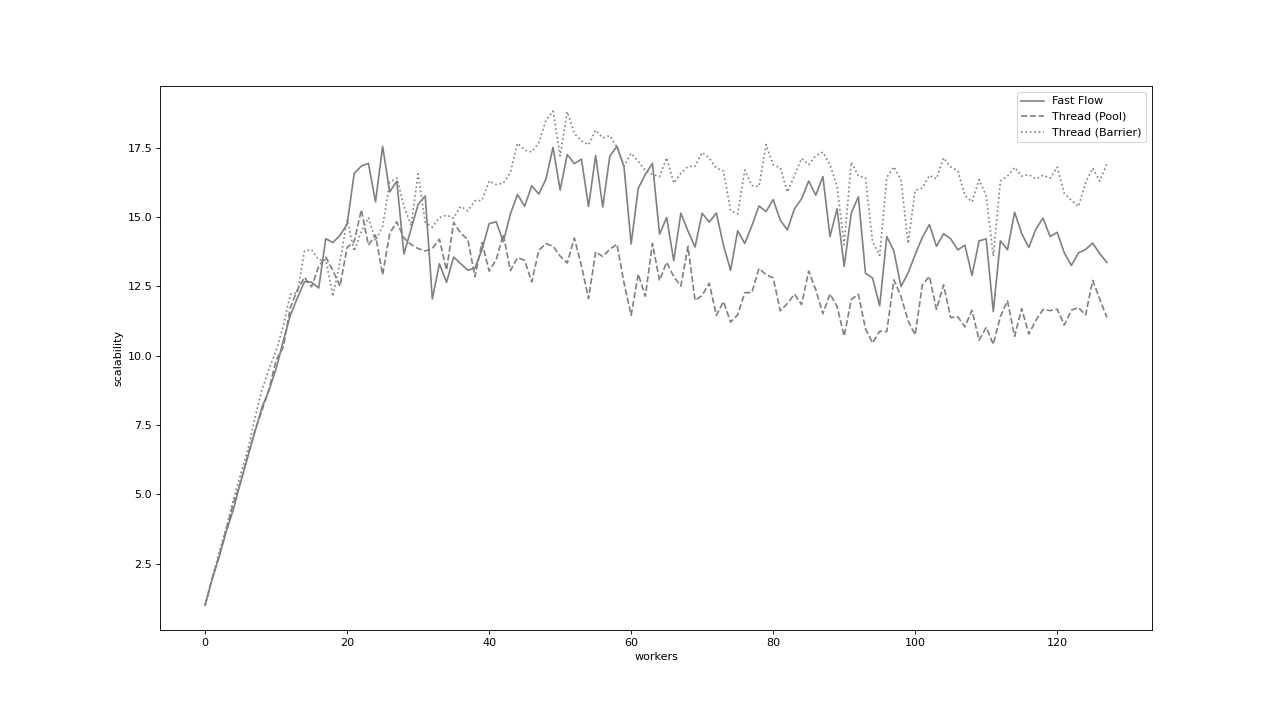
\includegraphics[width=18cm, center]{./plots/scalability_16384_1.png}
    \caption{Plot of scalability with n = 16384 with norm computation}
\end{figure} 

% --- EFFICIENCY

\begin{figure}[H]
\centering
    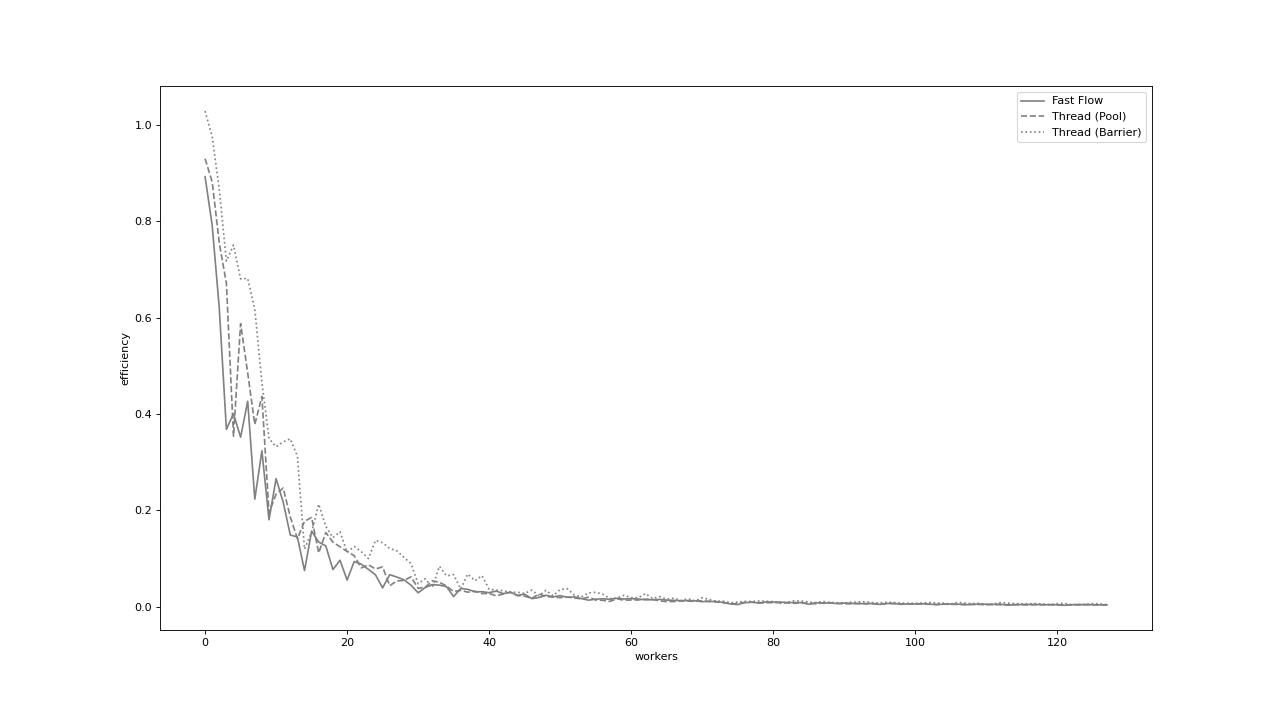
\includegraphics[width=18cm, center]{./plots/efficiency_1024_0.png}
    \caption{Plot of efficiency with n = 1024 without norm computation}
\end{figure}

\begin{figure}[H]
\centering
    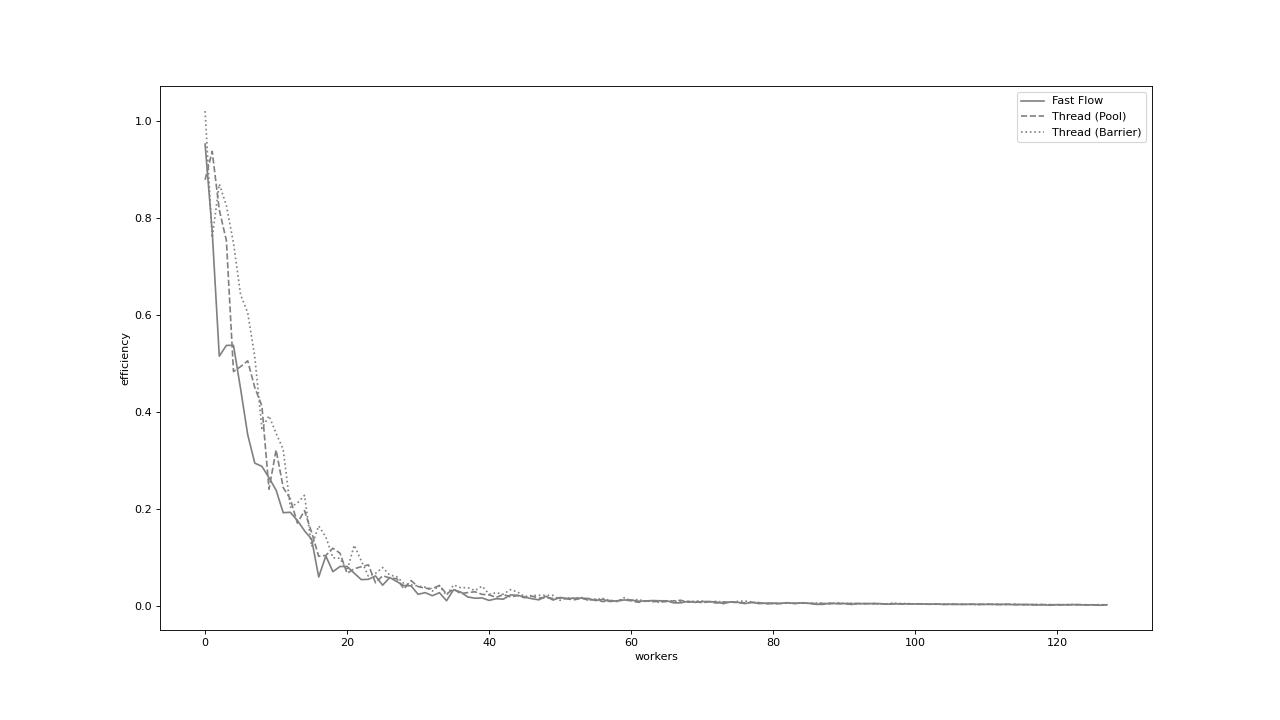
\includegraphics[width=18cm, center]{./plots/efficiency_1024_1.png}
    \caption{Plot of efficiency with n = 1024 with norm computation}
\end{figure} 

\begin{figure}[H]
\centering
    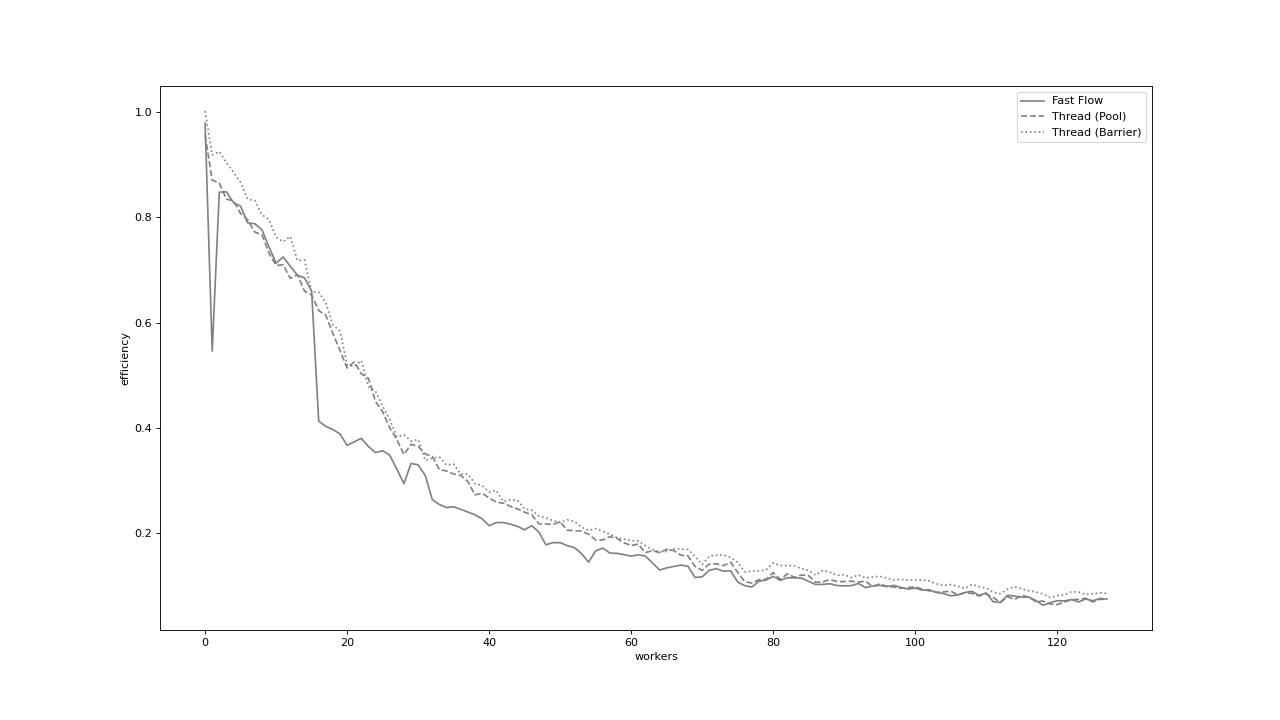
\includegraphics[width=18cm, center]{./plots/efficiency_16384_0.png}
    \caption{Plot of efficiency with n = 16384 without norm computation}
\end{figure} 


\begin{figure}[H]
\centering
    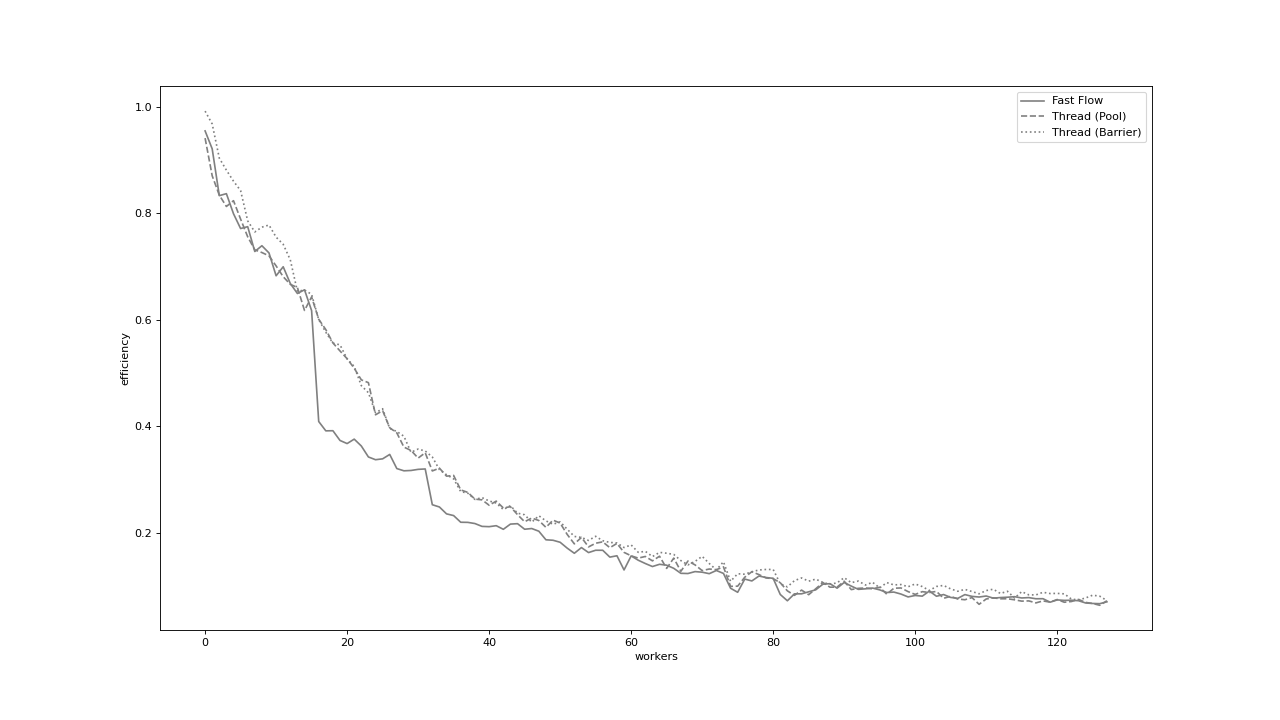
\includegraphics[width=18cm, center]{./plots/efficiency_16384_1.png}
    \caption{Plot of efficiency with n = 16384 with norm computation}
\end{figure}

\begin{table}[H]
\setlength{\tabcolsep}{10pt} % Default value: 6pt
\renewcommand{\arraystretch}{1.2} % Default value: 1
\centering
\begin{tabular}{|ccc|}
\hline
\multicolumn{1}{|c||}{Method}   & \multicolumn{1}{c|}{Number of workers $nw$}    & \multicolumn{1}{c|}{Time (micro seconds)} \\ \hline
\multicolumn{1}{|c||}{Fast Flow} & \multicolumn{1}{c|}{5} & \multicolumn{1}{c|}{3538.4} \\ \hline
\multicolumn{1}{|c||}{Threads (Pool)}       & \multicolumn{1}{c|}{9} & \multicolumn{1}{c|}{2560.0}  \\ \hline
\multicolumn{1}{|c||}{Threads (Barrier)} & \multicolumn{1}{c|}{7} & 
\multicolumn{1}{c|}{2246.0} \\ \hline
\end{tabular}
\caption{Result of the best timing and relative number of workers with norm computation for $N=1024$}
\end{table}

\begin{table}[H]
\setlength{\tabcolsep}{10pt} % Default value: 6pt
\renewcommand{\arraystretch}{1.2} % Default value: 1
\centering
\begin{tabular}{|ccc|}
\hline
\multicolumn{1}{|c||}{Method}   & \multicolumn{1}{c|}{Number of workers $nw$}    & \multicolumn{1}{c|}{Time (micro seconds)} \\ \hline
\multicolumn{1}{|c||}{Fast Flow} & \multicolumn{1}{c|}{7} & \multicolumn{1}{c|}{3896.4} \\ \hline
\multicolumn{1}{|c||}{Threads (Pool)}       & \multicolumn{1}{c|}{9} & \multicolumn{1}{c|}{2963.2}  \\ \hline
\multicolumn{1}{|c||}{Threads (Barrier)} & \multicolumn{1}{c|}{8} & 
\multicolumn{1}{c|}{2353.2} \\ \hline
\end{tabular}
\caption{Result of the best timing and relative number of workers without norm computation for $N=1024$}
\end{table}

\begin{table}[H]
\setlength{\tabcolsep}{10pt} % Default value: 6pt
\renewcommand{\arraystretch}{1.2} % Default value: 1
\centering
\begin{tabular}{|ccc|}
\hline
\multicolumn{1}{|c||}{Method}   & \multicolumn{1}{c|}{Number of workers $nw$}    & \multicolumn{1}{c|}{Time (micro seconds)} \\ \hline
\multicolumn{1}{|c||}{Fast Flow} & \multicolumn{1}{c|}{32} & \multicolumn{1}{c|}{147929.0} \\ \hline
\multicolumn{1}{|c||}{Threads (Pool)}       & \multicolumn{1}{c|}{24} & \multicolumn{1}{c|}{130848.2}  \\ \hline
\multicolumn{1}{|c||}{Threads (Barrier)} & \multicolumn{1}{c|}{32} & 
\multicolumn{1}{c|}{133812.6} \\ \hline
\end{tabular}
\caption{Result of the best timing and relative number of workers with norm computation for $N=16384$}
\end{table}

\begin{table}[H]
\setlength{\tabcolsep}{10pt} % Default value: 6pt
\renewcommand{\arraystretch}{1.2} % Default value: 1
\centering
\begin{tabular}{|ccc|}
\hline
\multicolumn{1}{|c||}{Method}   & \multicolumn{1}{c|}{Number of workers $nw$}    & \multicolumn{1}{c|}{Time (micro seconds)} \\ \hline
\multicolumn{1}{|c||}{Fast Flow} & \multicolumn{1}{c|}{16} & \multicolumn{1}{c|}{289320.2} \\ \hline
\multicolumn{1}{|c||}{Threads (Pool)}       & \multicolumn{1}{c|}{24} & \multicolumn{1}{c|}{257322.4}  \\ \hline
\multicolumn{1}{|c||}{Threads (Barrier)} & \multicolumn{1}{c|}{32} & 
\multicolumn{1}{c|}{251452.8} \\ \hline
\end{tabular}
\caption{Result of the best timing and relative number of workers without norm computation for $N=16384$}
\end{table}

\section{Conclusions}
So to conclude, we can notice that the theoretical based prespectives are turned to be true, since from the plots we can notice that, with $N=1024$ (low dimensionality) the time needed can't go to much low with higher $nw$, on the other hand with $N=16384$ (large dimensionality) we can reach a better speedup (and the other derived metrics), as the formulae said. On the other hand the differences in the speedup (and derived measures) between the run with norm and without norm computation is not to much, so is true that the proportion gained in serial fraction is not so huge to guarantee visible improvements.\\
Another point to highlight is that the experiment done can be expanded taking into account difference matrices, so we have tested over a single random matrix, and the tweaking of the parameters of the problem initialization, but I think that for the purpose of the exam this is sufficient.\\
The code, with the instruction to run and compile it, can be found here:\\ \href{https://github.com/Andrew-Wyn/SPM_Project}{https://github.com/Andrew-Wyn/SPM\_Project}

\bibliographystyle{plain}
\bibliography{bibliography.bib}
\end{document}